\chapter{Frequency-Shift Keying (FSK)}
\label{ch:fsk}

\begin{nontechnical}
\textbf{FSK is like Morse code with two different musical notes}---high note = 1, low note = 0. Simple, robust, and still used everywhere!

\textbf{Musical analogy:}
\begin{itemize}
\item Playing piano: \textbf{C note} = bit 0, \textbf{E note} = bit 1
\item Song: ``C C E C E E C'' = data: ``0 0 1 0 1 1 0''
\item Your ear (receiver) easily distinguishes C from E!
\item FSK receiver does the same with radio frequencies
\end{itemize}

\textbf{Why it's great:} Noise changes amplitude, but frequency stays clear! Immune to fading---signal can get weaker, but frequency doesn't change.

\textbf{Where you hear it:}
\begin{itemize}
\item \textbf{Caller ID}: Your phone uses FSK between rings
\item \textbf{Fax machines}: Those alternating tones you can hear
\item \textbf{Dial-up modems}: BEEEE-doo-BEEEE-doo (remember the 90s?)
\end{itemize}

\textbf{Modern uses:} Bluetooth Low Energy (GFSK), LoRa IoT networks, weather balloons, RFID tags.
\end{nontechnical}

\section{Overview}

\textbf{Frequency-Shift Keying (FSK)} is a digital modulation scheme where binary data is represented by switching between two discrete carrier frequencies.

\begin{keyconcept}
FSK provides \textbf{excellent immunity to amplitude variations} and \textbf{non-coherent detection capability}, making it ideal for harsh channel conditions, low-power applications, and simple receiver implementations.
\end{keyconcept}

Unlike phase-based modulation schemes (BPSK, QPSK), FSK encodes information in the \textbf{frequency domain}, allowing receivers to detect transmitted data without requiring precise carrier phase synchronization.

\section{Mathematical Description}

\subsection{Time-Domain Signal}

For binary FSK (BFSK), the transmitted signal for bit $n$ is:
\begin{equation}
s_n(t) = A \cos(2\pi f_n t), \quad 0 \leq t < T_b
\end{equation}
where:
\begin{itemize}
\item $A$ = constant carrier amplitude
\item $f_n \in \{f_0, f_1\}$ = transmitted frequency for bit $n$
\item $T_b$ = bit duration (seconds)
\end{itemize}

\textbf{Frequency encoding:}
\begin{equation}
f_n = \begin{cases}
f_0 & \text{if bit = 0 (``space'' frequency)} \\
f_1 & \text{if bit = 1 (``mark'' frequency)}
\end{cases}
\end{equation}

\subsection{General Form}

The FSK signal can be expressed as:
\begin{equation}
s(t) = A \cos\left[2\pi\left(f_c + b_k \cdot \frac{\Delta f}{2}\right)t\right]
\end{equation}
for $kT_b \leq t < (k+1)T_b$, where:
\begin{itemize}
\item $f_c$ = center carrier frequency (Hz)
\item $b_k \in \{-1, +1\}$ = bipolar data symbol
\item $\Delta f = f_1 - f_0$ = frequency separation (Hz)
\end{itemize}

\subsection{Modulation Index}

The \textbf{modulation index} characterizes the frequency deviation relative to the bit rate:
\begin{equation}
h = \frac{\Delta f \cdot T_b}{1} = \Delta f \cdot T_b = \frac{\Delta f}{R_b}
\end{equation}
where $R_b = 1/T_b$ is the bit rate (bps).

\textbf{Common values:}
\begin{itemize}
\item $h = 0.5$: Minimum Shift Keying (MSK)---narrowest orthogonal FSK
\item $h = 1.0$: Sunde's FSK---optimal orthogonality
\item $h > 1$: Wideband FSK---improved noise immunity, wider bandwidth
\end{itemize}

\begin{calloutbox}{Orthogonality Condition}
For \textbf{orthogonal FSK}, the two frequencies must satisfy:
\begin{equation}
\Delta f = \frac{n}{2T_b}, \quad n \in \mathbb{Z}^+
\end{equation}
Minimum orthogonal spacing: $\Delta f = \frac{1}{2T_b}$ (MSK, $h = 0.5$).

Orthogonal signals allow optimal non-coherent detection with minimal mutual interference.
\end{calloutbox}

\section{Spectral Characteristics}

\subsection{Bandwidth (Carson's Rule)}

The approximate bandwidth of FSK is given by \textbf{Carson's rule}:
\begin{equation}
B \approx 2(\Delta f + R_b) = 2R_b(h + 1)
\end{equation}
where:
\begin{itemize}
\item $\Delta f$ = frequency separation (Hz)
\item $R_b$ = bit rate (bps)
\item $h$ = modulation index
\end{itemize}

\textbf{Examples:}
\begin{itemize}
\item \textbf{MSK} ($h = 0.5$): $B \approx 1.5 R_b$ (most spectrally efficient FSK)
\item \textbf{Sunde's FSK} ($h = 1.0$): $B \approx 2 R_b$
\item \textbf{Wideband FSK} ($h = 2.0$): $B \approx 6 R_b$
\end{itemize}

The power spectral density consists of two main lobes centered at $f_0$ and $f_1$, with sidelobe amplitude depending on pulse shaping.

\section{Constellation Diagram}

Unlike phase-based modulation, FSK does not have a traditional I/Q constellation in the same sense. However, for orthogonal coherent FSK, we can represent the two signals as orthogonal vectors:

\begin{center}
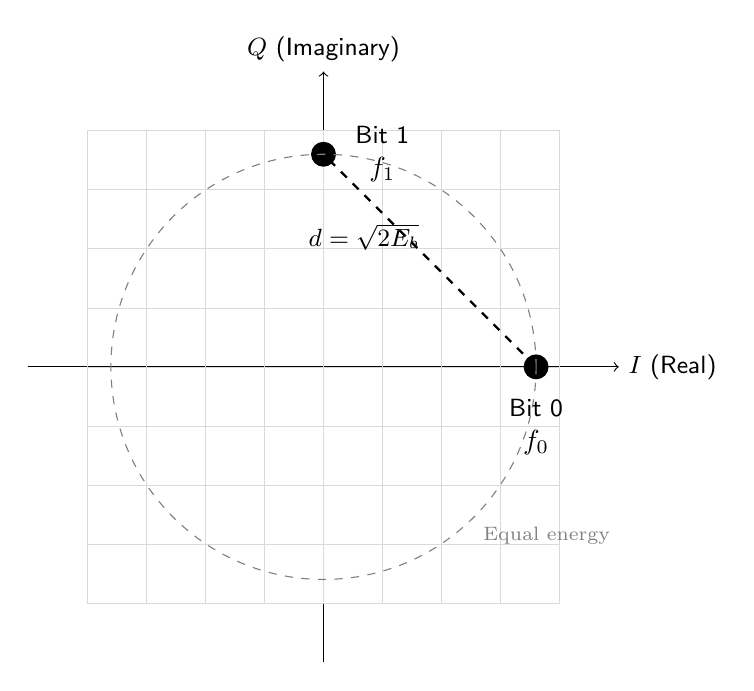
\begin{tikzpicture}[scale=1.5]
% Axes
\draw[->] (-2.5,0) -- (2.5,0) node[right] {\sffamily\small $I$ (Real)};
\draw[->] (0,-2.5) -- (0,2.5) node[above] {\sffamily\small $Q$ (Imaginary)};

% Grid
\draw[very thin,gray!30] (-2,-2) grid[step=0.5] (2,2);

% Constellation points for orthogonal FSK
\fill[black] (1.8,0) circle (3pt);
\fill[black] (0,1.8) circle (3pt);

% Labels
\node[below=8pt,align=center] at (1.8,0) {\sffamily\small Bit 0\\$f_0$};
\node[right=8pt,align=center] at (0,1.8) {\sffamily\small Bit 1\\$f_1$};

% Distance annotation
\draw[<->,thick,dashed] (1.8,0) -- (0,1.8) node[midway,above left] {\sffamily\small $d = \sqrt{2E_b}$};

% Energy circle
\draw[thin,gray,dashed] (0,0) circle (1.8);
\node[below right,gray,font=\scriptsize] at (1.27,-1.27) {Equal energy};
\end{tikzpicture}
\end{center}

For \textbf{orthogonal FSK}, the two signal vectors are perpendicular (90° apart), providing:
\begin{equation}
d = \sqrt{2E_b}
\end{equation}
where $E_b = A^2T_b/2$ is the energy per bit.

\section{Modulation and Demodulation}

\subsection{Transmitter (Modulator)}

The FSK modulator can be implemented using frequency synthesis:

\begin{center}
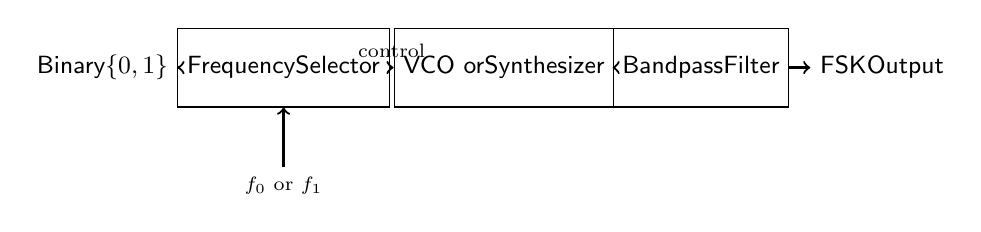
\begin{tikzpicture}[
  block/.style={rectangle, draw, minimum width=2cm, minimum height=1cm, font=\sffamily\small},
  node distance=2cm,
  font=\small
]
\node (input) {\sffamily Binary\\$\{0, 1\}$};
\node[block, right of=input, node distance=2.3cm] (switch) {Frequency\\Selector};
\node[block, right of=switch, node distance=2.8cm] (vco) {VCO or\\Synthesizer};
\node[block, right of=vco, node distance=2.5cm] (filter) {Bandpass\\Filter};
\node[right of=filter, node distance=2.3cm] (output) {\sffamily FSK\\Output};

\node[below of=switch, node distance=1.5cm, font=\scriptsize, align=center] (freq) {$f_0$ or $f_1$};

\draw[->,thick] (input) -- (switch);
\draw[->,thick] (switch) -- node[above,font=\scriptsize] {control} (vco);
\draw[->,thick] (vco) -- (filter);
\draw[->,thick] (filter) -- (output);
\draw[->,thick] (freq) -- (switch);
\end{tikzpicture}
\end{center}

\textbf{Process:}
\begin{enumerate}
\item \textbf{Data bit determines frequency:} Bit 0 $\rightarrow$ $f_0$, Bit 1 $\rightarrow$ $f_1$
\item \textbf{Voltage-Controlled Oscillator (VCO):} Generates carrier at selected frequency
\item \textbf{Bandpass filter:} Shapes spectrum and removes harmonics
\end{enumerate}

\subsection{Receiver: Non-Coherent Detection}

The most common FSK demodulation uses \textbf{non-coherent detection}, which does not require carrier phase synchronization:

\begin{center}
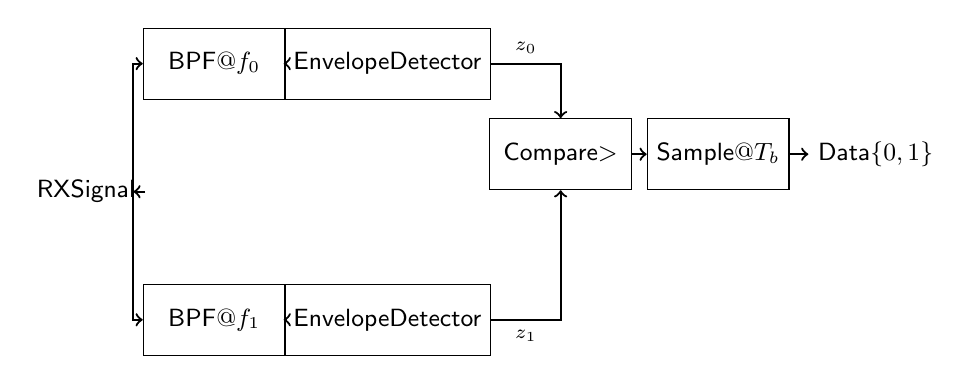
\begin{tikzpicture}[
  block/.style={rectangle, draw, minimum width=1.8cm, minimum height=0.9cm, font=\sffamily\small},
  node distance=1.8cm,
  font=\small
]
\node (input) {\sffamily RX\\Signal};
\node[block, above right of=input, node distance=2.3cm] (bpf0) {BPF\\$@f_0$};
\node[block, right of=bpf0, node distance=2.2cm] (env0) {Envelope\\Detector};
\node[block, below right of=input, node distance=2.3cm] (bpf1) {BPF\\$@f_1$};
\node[block, right of=bpf1, node distance=2.2cm] (env1) {Envelope\\Detector};
\node[block, right of=env0, node distance=2.2cm, yshift=-1.15cm] (comp) {Compare\\$>$};
\node[block, right of=comp, node distance=2cm] (sample) {Sample\\$@T_b$};
\node[right of=sample, node distance=2cm] (output) {\sffamily Data\\$\{0,1\}$};

\draw[->,thick] (input) -- ++(0.6,0) coordinate (split);
\draw[->,thick] (split) |- (bpf0);
\draw[->,thick] (split) |- (bpf1);
\draw[->,thick] (bpf0) -- (env0);
\draw[->,thick] (bpf1) -- (env1);
\draw[->,thick] (env0) -| node[near start,above,font=\scriptsize] {$z_0$} (comp);
\draw[->,thick] (env1) -| node[near start,below,font=\scriptsize] {$z_1$} (comp);
\draw[->,thick] (comp) -- (sample);
\draw[->,thick] (sample) -- (output);
\end{tikzpicture}
\end{center}

\textbf{Detection process:}
\begin{enumerate}
\item \textbf{Bandpass filters:} Separate $f_0$ and $f_1$ components
\item \textbf{Envelope detectors:} Measure signal amplitude in each channel
\item \textbf{Compare:} Select channel with larger envelope
\item \textbf{Decision:} If $z_0 > z_1$: bit = 0; else: bit = 1
\end{enumerate}

\begin{keyconcept}
\textbf{Non-coherent detection} eliminates the need for carrier phase recovery, significantly simplifying receiver design. The performance penalty is approximately \textbf{1~dB} compared to coherent detection---a worthwhile trade-off for many applications.
\end{keyconcept}

\subsection{Coherent Detection (Optimal)}

For maximum performance, coherent detection uses correlation receivers:

\begin{center}
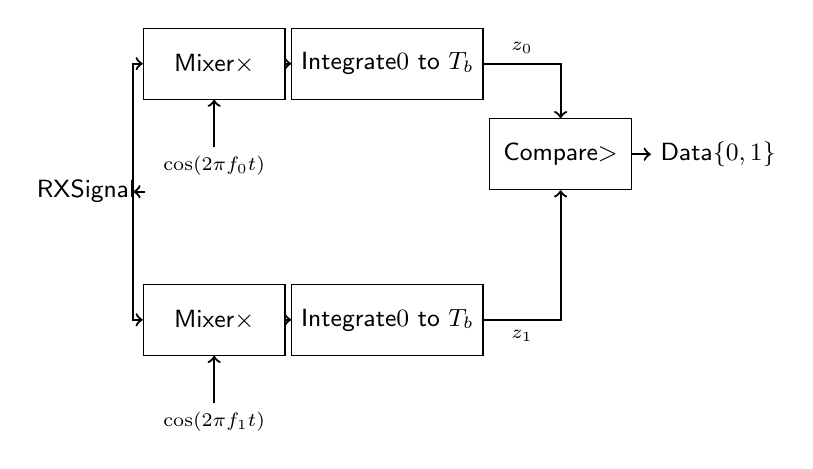
\begin{tikzpicture}[
  block/.style={rectangle, draw, minimum width=1.8cm, minimum height=0.9cm, font=\sffamily\small},
  node distance=1.8cm,
  font=\small
]
\node (input) {\sffamily RX\\Signal};
\node[block, above right of=input, node distance=2.3cm] (mult0) {Mixer\\$\times$};
\node[block, right of=mult0, node distance=2.2cm] (int0) {Integrate\\$0$ to $T_b$};
\node[block, below right of=input, node distance=2.3cm] (mult1) {Mixer\\$\times$};
\node[block, right of=mult1, node distance=2.2cm] (int1) {Integrate\\$0$ to $T_b$};
\node[block, right of=int0, node distance=2.2cm, yshift=-1.15cm] (comp) {Compare\\$>$};
\node[right of=comp, node distance=2cm] (output) {\sffamily Data\\$\{0,1\}$};

\node[below of=mult0, node distance=1.3cm, font=\scriptsize, align=center] (lo0) {$\cos(2\pi f_0 t)$};
\node[below of=mult1, node distance=1.3cm, font=\scriptsize, align=center] (lo1) {$\cos(2\pi f_1 t)$};

\draw[->,thick] (input) -- ++(0.6,0) coordinate (split);
\draw[->,thick] (split) |- (mult0);
\draw[->,thick] (split) |- (mult1);
\draw[->,thick] (lo0) -- (mult0);
\draw[->,thick] (lo1) -- (mult1);
\draw[->,thick] (mult0) -- (int0);
\draw[->,thick] (mult1) -- (int1);
\draw[->,thick] (int0) -| node[near start,above,font=\scriptsize] {$z_0$} (comp);
\draw[->,thick] (int1) -| node[near start,below,font=\scriptsize] {$z_1$} (comp);
\draw[->,thick] (comp) -- (output);
\end{tikzpicture}
\end{center}

\textbf{Coherent detection provides optimal performance but requires:}
\begin{itemize}
\item Precise local oscillators at both $f_0$ and $f_1$
\item Phase synchronization (approx.\ 1~dB improvement over non-coherent)
\item More complex receiver circuitry
\end{itemize}

\begin{warningbox}
\textbf{Frequency accuracy is critical.} The local oscillators must match the transmitter frequencies exactly. Even small frequency offsets degrade performance. For non-coherent FSK, frequency stability requirements are relaxed compared to phase-coherent modulation schemes like BPSK.
\end{warningbox}

\section{Bit Error Rate (BER) Performance}

\subsection{Non-Coherent FSK in AWGN Channel}

For orthogonal non-coherent FSK with envelope detection:
\begin{equation}
\mathrm{BER} = \frac{1}{2}e^{-E_b/(2N_0)}
\end{equation}
where:
\begin{itemize}
\item $E_b = \frac{A^2 T_b}{2}$ = energy per bit (joules)
\item $N_0$ = noise power spectral density (W/Hz)
\end{itemize}

\subsection{Coherent FSK in AWGN Channel}

For orthogonal coherent FSK with correlation detection:
\begin{equation}
\mathrm{BER} = Q\left(\sqrt{\frac{E_b}{N_0}}\right) = \frac{1}{2}\mathrm{erfc}\left(\sqrt{\frac{E_b}{2N_0}}\right)
\end{equation}

\textbf{Performance benchmarks:}

\begin{center}
\begin{tabular}{@{}lrrl@{}}
\toprule
$E_b/N_0$ (dB) & \multicolumn{1}{c}{BER (Non-coh)} & \multicolumn{1}{c}{BER (Coherent)} & Practical Meaning \\
\midrule
5~dB & $6.7 \times 10^{-2}$ & $3.9 \times 10^{-2}$ & 1 error in 15--25 bits \\
10~dB & $6.7 \times 10^{-4}$ & $1.9 \times 10^{-4}$ & 1 error in 1,500--5,000 bits \\
12~dB & $1.2 \times 10^{-4}$ & $2.6 \times 10^{-5}$ & 1 error in 8,000--38,000 bits \\
15~dB & $3.7 \times 10^{-6}$ & $4.3 \times 10^{-7}$ & 1 error in $270$k--$2.3$M bits \\
\bottomrule
\end{tabular}
\end{center}

\textbf{Key insight:} Coherent detection provides approximately \textbf{1~dB} advantage over non-coherent detection at practical BER levels.

\subsection{Comparison with Other Modulation Schemes}

\begin{center}
\small
\begin{tabular}{@{}lcccc@{}}
\toprule
\textbf{Scheme} & \textbf{Spectral Eff.} & \textbf{$E_b/N_0$} & \textbf{Complex.} & \textbf{Detection} \\
 & \textbf{(bps/Hz)} & \textbf{@ BER $10^{-6}$} & & \\
\midrule
OOK & $\sim$0.5 & 13.5~dB & Low & Non-coh. \\
\textbf{FSK (non-coh)} & $\sim$0.5 & 12.5~dB & Low & Non-coh. \\
\textbf{FSK (coherent)} & $\sim$0.5 & 10.5~dB & Medium & Coherent \\
MSK & $\sim$0.67 & 10.5~dB & Medium & Coherent \\
BPSK & $\sim$1.0 & 10.5~dB & Medium & Coherent \\
QPSK & $\sim$2.0 & 10.5~dB & Medium & Coherent \\
\bottomrule
\end{tabular}
\end{center}

\section{Worked Example: LoRa IoT Link Budget}

\begin{calloutbox}{Example: LoRa FSK Link at 915~MHz}

\textbf{Scenario:} Agricultural sensor transmitting to gateway 5~km away

\subsection*{Given Parameters}

\begin{tabular}{@{}ll@{}}
TX power & $P_t = 14$~dBm (25~mW) \\
TX antenna gain & $G_t = 2$~dBi (omnidirectional) \\
Distance & $d = 5$~km \\
Frequency & $f = 915$~MHz (ISM band) \\
RX antenna gain & $G_r = 6$~dBi (directional) \\
Receiver noise figure & $NF = 6$~dB \\
Bandwidth & $B = 125$~kHz (LoRa BW) \\
Data rate & $R_b = 1$~kbps \\
Required BER & $10^{-3}$ \\
\end{tabular}

\subsection*{Solution}

\textbf{Step 1: Free-Space Path Loss}
\begin{equation}
\mathrm{FSPL} = 20\log_{10}(5) + 20\log_{10}(915) + 32.45 = 113.6~\text{dB}
\end{equation}

\textbf{Step 2: Received Power}
\begin{equation}
P_r = 14 + 2 + 6 - 113.6 = -91.6~\text{dBm}
\end{equation}

\textbf{Step 3: Noise Power}

Thermal noise: $N_0 = -174$~dBm/Hz

Noise power: $N = -174 + 10\log_{10}(125{,}000) + 6 = -117~\text{dBm}$

\textbf{Step 4: SNR and $E_b/N_0$}
\begin{equation}
\mathrm{SNR} = -91.6 - (-117) = 25.4~\text{dB}
\end{equation}
\begin{equation}
\frac{E_b}{N_0} = 25.4 + 10\log_{10}\left(\frac{125{,}000}{1{,}000}\right) = 25.4 + 21 = 46.4~\text{dB}
\end{equation}

\textbf{Step 5: Link Margin}

Required $E_b/N_0$ for FSK @ BER $10^{-3}$: $\sim$8~dB

Link margin: $46.4 - 8 = 38.4$~dB (excellent!)

\textbf{Conclusion:} Massive link margin allows for multipath fading, foliage attenuation, and other impairments typical in IoT deployments.
\end{calloutbox}

\section{Advantages and Disadvantages}

\subsection*{Advantages}

\begin{enumerate}
\item \textbf{Constant envelope:} Power amplifiers can operate in saturation (Class C) with maximum efficiency
\item \textbf{Non-coherent detection:} Simple receivers without carrier recovery loops
\item \textbf{Amplitude immunity:} Robust against fading and amplitude variations
\item \textbf{Frequency discrimination:} Easier than phase detection in noisy channels
\item \textbf{Low-cost implementation:} VCO-based modulators are inexpensive
\item \textbf{Legacy compatibility:} Widely deployed in existing systems
\end{enumerate}

\subsection*{Disadvantages}

\begin{enumerate}
\item \textbf{Poor spectral efficiency:} Requires $\sim$2$\times$ bandwidth of PSK schemes
\item \textbf{Moderate power efficiency:} 1--2~dB worse than coherent BPSK
\item \textbf{Frequency stability:} Requires accurate oscillators (especially for narrowband)
\item \textbf{Doppler sensitivity:} Frequency offsets degrade performance
\item \textbf{Lower data rates:} Not suitable for high-throughput applications
\end{enumerate}

\section{Practical Applications}

\subsection{Historical Systems}

\subsubsection{Telephone Modems}

\begin{itemize}
\item \textbf{Bell 103 (1962):} 300~bps, $f_0 = 1070$~Hz, $f_1 = 1270$~Hz
\item \textbf{Bell 202 (1976):} 1200~bps, $f_0 = 2200$~Hz, $f_1 = 1200$~Hz (still used for caller ID)
\item \textbf{V.21 (CCITT):} 300~bps full-duplex over phone lines
\end{itemize}

\subsubsection{Radio Communication}

\begin{itemize}
\item \textbf{Radio Teletype (RTTY):} HF radio, 45.45~baud, $\Delta f = 170$~Hz (still used by amateur radio)
\item \textbf{Pagers:} POCSAG (1981), FLEX (1993)---millions deployed worldwide
\item \textbf{Emergency broadcasts:} Weather radio, emergency alert system (EAS) tones
\end{itemize}

\subsection{Modern IoT and Wireless Systems}

\subsubsection{LoRa (Long Range)}

\begin{itemize}
\item \textbf{Technology:} Chirp Spread Spectrum (CSS) FSK variant
\item \textbf{Frequency bands:} 433~MHz, 868~MHz (EU), 915~MHz (US)
\item \textbf{Range:} Up to 15~km rural, 2--5~km urban
\item \textbf{Data rates:} 0.3--50~kbps (adaptive)
\item \textbf{Applications:} Smart agriculture, asset tracking, smart cities
\end{itemize}

\subsubsection{Bluetooth Low Energy (BLE)}

\begin{itemize}
\item \textbf{Modulation:} GFSK (Gaussian FSK)
\item \textbf{Modulation index:} $h = 0.5$ (MSK)
\item \textbf{Data rate:} 1~Mbps (BLE 4.x), 2~Mbps (BLE 5.0)
\item \textbf{Applications:} Wearables, beacons, smart home devices
\end{itemize}

\subsubsection{IEEE 802.15.4 (Zigbee)}

\begin{itemize}
\item \textbf{Bands:} 868~MHz (Europe), 915~MHz (Americas), 2.4~GHz (worldwide)
\item \textbf{Modulation:} BPSK (sub-GHz), O-QPSK (2.4~GHz)
\item \textbf{Related:} Thread, 6LoWPAN protocols
\end{itemize}

\subsection{Specialized Applications}

\begin{itemize}
\item \textbf{RFID systems:} Passive tags use FSK backscatter
\item \textbf{Weather balloons:} Radiosondes transmit meteorological data via FSK (400~MHz)
\item \textbf{Wireless sensor networks:} Low-power nodes with simple FSK trans\-ceiv\-ers
\item \textbf{Submarine communication:} VLF/ELF FSK for underwater links
\end{itemize}

\section{FSK Variants}

\subsection{Minimum Shift Keying (MSK)}

Special case where $h = 0.5$ (minimum for orthogonality):

\begin{itemize}
\item \textbf{Continuous phase:} No phase discontinuities at bit boundaries
\item \textbf{Constant envelope:} Ideal for nonlinear amplifiers
\item \textbf{Bandwidth:} $B \approx 1.5 R_b$ (narrowest orthogonal FSK)
\item \textbf{Equivalent form:} Offset QPSK with half-sine pulse shaping
\item \textbf{Used in:} GSM cellular (GMSK variant), satellite communications
\end{itemize}

\subsection{Gaussian FSK (GFSK)}

MSK with Gaussian pre-modulation filtering:

\begin{itemize}
\item \textbf{Purpose:} Reduce spectral sidelobes for tighter spectrum occupancy
\item \textbf{BT product:} $B \times T_b$ typically 0.3--0.5
\item \textbf{Bandwidth:} $B \approx 1.2$--$1.5 R_b$ depending on BT
\item \textbf{Applications:} Bluetooth (BT = 0.5), Zigbee, DECT
\end{itemize}

\subsection{Continuous Phase FSK (CPFSK)}

Phase is continuous across all bit boundaries:
\begin{equation}
\phi(t) = 2\pi\left[f_c t + \frac{h\Delta f}{2}\int_0^t b(\tau)\,d\tau\right]
\end{equation}

\textbf{Benefits:}
\begin{itemize}
\item No spectral splatter from phase jumps
\item Improved spectral efficiency
\item Smoother power envelope
\end{itemize}

\subsection{Multi-Frequency FSK (MFSK)}

Uses $M > 2$ frequencies for higher order modulation:

\begin{itemize}
\item \textbf{Symbol encoding:} $\log_2(M)$ bits per symbol
\item \textbf{Example (4-FSK):} $f_0, f_1, f_2, f_3$ encode 00, 01, 10, 11
\item \textbf{Bandwidth:} $B \approx M \cdot R_s$ (wider than binary FSK)
\item \textbf{Power efficiency:} Better than BFSK at high $M$ and low SNR
\item \textbf{Applications:} HF radio (MT63, Olivia), meteor scatter
\end{itemize}

\section{Summary}

\begin{center}
\begin{tabular}{@{}ll@{}}
\toprule
\textbf{Parameter} & \textbf{Value} \\
\midrule
Bits per symbol & 1 (binary FSK) \\
Modulation method & Frequency switching \\
Typical bandwidth (Carson) & $\sim$2$R_b$ (non-coherent) \\
Spectral efficiency & $\sim$0.5~bps/Hz \\
BER @ 12~dB $E_b/N_0$ (non-coh) & $1.2 \times 10^{-4}$ \\
BER @ 12~dB $E_b/N_0$ (coherent) & $2.6 \times 10^{-5}$ \\
Detection type & Non-coherent or coherent \\
Carrier recovery & Not required (non-coherent) \\
Envelope & Constant \\
Implementation & Simple (VCO-based) \\
Best application & Low-power, harsh channels, IoT \\
Typical uses & LoRa, Bluetooth (GFSK), caller ID, pagers \\
\bottomrule
\end{tabular}
\end{center}

\textbf{Key advantages:}
\begin{itemize}
\item Robust amplitude immunity
\item Simple non-coherent detection
\item Constant envelope for efficient amplifiers
\item Proven technology with wide deployment
\end{itemize}

\textbf{Key trade-offs:}
\begin{itemize}
\item Lower spectral efficiency than PSK/QAM
\item Wider bandwidth requirement
\item Moderate power efficiency (1--2~dB penalty vs BPSK)
\end{itemize}

\section{Further Reading}

\begin{itemize}
\item \textbf{Chapter~\ref{ch:bpsk}:} Binary Phase-Shift Keying (BPSK)---coherent alternative with better spectral efficiency
\item \textbf{Chapter~5:} On-Off Keying (OOK)---simpler amplitude modulation
\item \textbf{Chapter~7:} Quadrature Phase-Shift Keying (QPSK)---2 bits/symbol extension
\item \textbf{Chapter~10:} Minimum Shift Keying (MSK)---optimal continuous-phase FSK
\item \textbf{Chapter~12:} Constellation Diagrams---modulation scheme visualization
\item \textbf{Chapter~13:} IQ Representation---complex baseband mathematics
\item \textbf{Chapter~18:} Bit Error Rate Analysis---performance measurement
\item \textbf{Chapter~22:} Forward Error Correction---coding for BER improvement
\item \textbf{Chapter~28:} Spread Spectrum Techniques---frequency hopping and chirp modulation
\item \textbf{Chapter~35:} IoT Communication Systems---LoRa, Sigfox, NB-IoT applications
\end{itemize}
